\documentclass[a4paper,10pt]{article}
\usepackage[utf8x]{inputenc}
\usepackage{multirow}
\usepackage{indentfirst}
\usepackage{graphicx}
\usepackage{amsmath}
\usepackage[version=3]{mhchem}
\usepackage{siunitx}
\usepackage{float}
\usepackage{subfigure}
\usepackage{morefloats}
\usepackage[pdftex]{hyperref}	%este tiene que ser el último usepackage en incluír?

\hypersetup{colorlinks = true}

\graphicspath{ 
	{../../celula/scripts/itvs/}
	{../../celula/scripts/curvas/}
	{../../celula/scripts/poros/}
	{../../mesh/AutoMesh2D/grande/}
}

%opening
\title{Modelado de Electroporación Celular}
\author{Mauricio Alfonso}

\begin{document}

\newcommand{\h}{\ce{H^+}}
\newcommand{\oh}{\ce{OH^-}}
\newcommand{\na}{\ce{Na^+}}
\newcommand{\cl}{\ce{Cl^-}}
\newcommand{\kvm}{$\si{\kilo\volt\per\metre}$}
\newcommand{\usec}{$\si{\micro\second}$}

%TODO bibliografía!! abs y zinter

\maketitle

%\begin{abstract}
%
%\end{abstract}
%
%
%\newpage

\section{Introducción}
%completa para después, pero primero explicar brevemente motivos que nos guían, etc
%explicar electroporación

La electroporación reversible es un método consistente en la aplicación de pulsos eléctricos de alta intensidad a una célula con el objetivo de permeabilizar su membrana creando poros, y así permitir el ingreso de drogas o moléculas de ADN a su interior. Esto permite tratar tumores con menores cantidades de drogas, reduciendo los efectos secundarios.\\

%TODO BIBLIO LOW algo de electroporation

%tipos de tratamientos ?

%lo que se hace en este trabajo
En este trabajo se simula una célula esférica a la que se le aplica un pulso eléctrico de 20\si{\milli\second} de duración a través de dos electrodos, y se estudia el ingreso al interior de la célula de 4 especies iónicas: el ión hidrógeno (\h), el hidróxido (\oh), el catión sodio (\na) y el cloruro (\cl). Para eso se tiene en cuenta el campo eléctrico producido por los electrodos, la generación y evolución de poros en la membrana celular producto de la diferencia de potencial entre el interior y exterior de la célula , y la migración de las especies mencionadas, producto de la diferencia de potencial.\\

%TODO mencionar que la densidad se calcula en distintas regiones

Las simulaciones se realizaron con el método de elementos finitos sobre mallas bidimensionales que representan el dominio sobre un sistema de coordenadas cilíndricas usando elementos cuadrilaterales.

%Se utiliza el método de elementos finitos para simular tres procesos? físicos diferentes: potencial eléctrico, generación de poros y transporte de especies, que se acoplan ???

%El trabajo está basado en otros ??? que realizan algunas de las mismas ecuaciones de manera separada

\clearpage
\section{Teoría}
%donde van todoas las ecuaciones y teoria

\subsection{Potencial eléctrico}

El campo eléctrico en el dominio es generado por dos electrodos con un potencial constante durante la duración del pulso. El potencial eléctrico en todo el dominio se calcula según la ecuación 

\begin{equation} \label{eq:poisson}
	\nabla \sigma_{elem} \cdot (\nabla \phi) = 0 
\end{equation}

donde $\phi$ representa el potencial eléctrico y $\sigma_{elem}$ la conductividad del material \cite[p.~88]{fem-electro}.\\

Para los bordes ocupados por los electrodos se usan condiciones de borde de Dirichlet con potenciales fijos, mientras que para los bordes no ocupados por electrodos se usan condiciones de borde de Neumann:

\begin{equation}
	\frac{\partial \phi}{\partial \mathbf{n}} = 0
\end{equation}

donde $\mathbf{n}$ representa la normal al borde.\\

La diferencia de potencial entre el interior y el exterior de la célula en un punto de su superficie se conoce como potencial transmembrana (ITV). Si la célula es esférica este potencial se puede aproximar de manera independiente del tiempo como

\begin{equation} \label{eq:cos}
	V^{\theta} = 1.5\, E\, \alpha\, cos (\theta)
\end{equation}

donde $E$ es el campo eléctrico, $\theta$ el ángulo polar respecto del campo eléctrico y $\alpha$ el radio de la célula \cite{puchiar}. Esta fórmula no tiene en cuenta que el ITV puede variar en el tiempo por la creación de poros, por eso en este trabajo no se la usa directamente, si no que usan las ecuaciones diferenciales. 

\subsection{Transporte de especies}
Para el transporte de especies se usa la ecuación de conservación de masa de Nernst-Planck:

\begin{equation} \label{eq:trans}
	\frac{\partial C_i}{\partial t} = \nabla \cdot \left( D_i \nabla C_i + D_i z_i \frac{F}{R T} C_i \nabla \phi \right)
\end{equation}

donde $C_i$, $D_i$ y $z_i$ representan la concentración, el coeficiente de difusión y la valencia 
respectivamente de la especie $i$, para $i = $ \h, \oh, \na ó \cl.
$F$ es la constante de Faraday, $R$ la constante de los gases y $T$ la temperatura \cite{fodava}. 
Esta ecuación tiene en cuenta la difusión de las partículas pero también el efecto que puede tener el campo eléctrico.\\

Como condiciones iniciales se usan las concentraciones descritas en la tabla \ref{table:tablita}: $C_{e, i}^0$ siendo $e =$ $i$ ó $o$ si se refiere a los nodos del interior o del exterior de la célula respectivamente e $i =$ \h, \oh, \na ó \cl para la concentración de cada especie y $C_{e,i}$ con $e =$ $a$ ó $c$ si es para el ánodo o el cátodo respectivamente.\\

Como condición de borde en el borde no ocupado por los electrodos se usa
\begin{equation}
	\frac{\partial C_i}{\partial \mathbf{n}} = 0
\end{equation}

Para los bordes ocupados por los electrodos se usan los valores fijos $C_{e,i}$ descritos anteriormente.

%donde $C_i$ representa la concentración de la especie $i$, $D_i$ el coeficiente de difusión de la 
%especie $i$, $z_i$ la valencia de la especie $i$, $F$ la constante de Faraday, $R$ la constante de los gases y $T$ la temperatura. Esta ecuación tiene en cuenta la difusión de las partículas pero también el efecto que puede tener el campo eléctrico.\\

%TODO explicar un poco más de esta ecuación

\subsection{Generación de poros}
Con el ITV se crean poros hidrofílicos en la membrana. La densidad de poros se calcula según la ecuación diferencial  

\begin{equation} \label{eq:poros-crea}
	\frac{\partial N}{\partial t} = \alpha_c e^{(V_m/V_{ep})^2} \left( 1 - \frac{N}{N_0 e^{q \left(V_m/V_{ep} \right) ^2}} \right)
\end{equation}

donde $N$ es la densidad de poros en un determinado tiempo y posición de la membrana celular, $\alpha_c$ es el coeficiente de creación de poros, $V_m$ es el potencial transmembrana, $V_{ep}$ es el voltaje característico de electroporación, $N_0$ es la densidad de poros en equilibrio (cuando $V_m = 0$) y $q$ es una constante igual a $(r_m / r*)^2$, donde $r_m$ es el radio de mínima energía para $V_m = 0$ y $r*$ es el radio mínimo de los poros \cite{krass}.\\

Los poros se crean con un radio inicial $r*$ y su radio varía en el tiempo según el potencial transmembrana de acuerdo a la ecuación diferencial

\begin{equation} \label{eq:poros-radio}
	\frac{\partial r}{\partial t} = \frac{D}{kT} \left( \frac{V_m^2 F_{max}}{1+r_h / (r+r_a)} + \frac{4 \beta}{r} \left(\frac{r_*}{r}\right)^4 - 2 \pi \gamma + 2 \pi \sigma_{\textrm{\tiny eff}} r\right)
\end{equation}

donde $r$ es el radio de un poro, $D$ es el coeficiente de difusión para los poros, $k$ es la constante de Boltzmann, $T$ la temperatura absoluta, $V_m$ el potencial transmembrana, $F_{max}$ la máxima fuerza eléctrica para $V_m$ de 1V, $r_h$ y $r_a$ son constantes usadas para la velocidad de advección, $\beta$ es la energía de repulsión estérica, $\gamma$ es la energía del perímetro de los poros, y $\sigma_{\textrm{\tiny eff}}$ es la tensión efectiva de la membrana, calculada como

\begin{equation}
	\sigma_{\textrm{\tiny eff}} = 2 \sigma^\prime - \frac{2 \sigma^\prime - \sigma_0}{(1 - A_p / A)^2}
\end{equation}

donde $\sigma^\prime$ es la tensión de la interfase hidrocarburo-agua, $\sigma_0$ es la tensión de la bicapa sin poros, $A_p$ es la suma de las áreas de todos los poros en la célula, y $A$ es el área de la célula \cite{krass}. En la ecuación \ref{eq:poros-radio}, el primer término corresponde a la fuerza eléctrica inducida por el potencial transmembrana, el segundo a la repulsión estérica, el tercero a la tensión de línea que actúa en el perímetro del poro y el cuarto a la tensión superficial de la célula\\

Por otra parte se asume que la membrana celular se carga como un capacitor y una resistencia en paralelo. De esta manera el potencial transmembrana no aumenta bruscamente al iniciarse el pulso eléctrico, si no que crece de manera paulatina según la ecuación: 

\begin{equation} \label{eq:capacit} \begin{split}
	V_m = V_p\, (1 - e^{-t/\tau}) , \\ \textrm{con } \tau = \alpha\, C_m \left( \frac{1}{\sigma_i} + \frac{1}{2 \sigma_o} \right)
\end{split} \end{equation}

donde $V_m$ es el potencial transmembrana en un punto de la superficie de la célula, $V_p$ es el potencial obtenido por las ecuaciones de potencial eléctrico en ése mismo punto, $t$ es el tiempo transcurrido desde el comienzo del pulso eléctrico, $\alpha$ es el radio de la célula, $C_m$ es la capacitancia superficial de la célula y $\sigma_i$ y $\sigma_o$ las conductancias intra y extracelulares respectivamente \cite{krass}.\\

\subsection{Método de Elementos Finitos}
El método de elementos finitos (FEM) sirve para resolver ecuaciones diferenciales de manera aproximada, discretizando el dominio en zonas pequeñas y disjuntas llamadas elementos, y resolviendo un sistema de ecuaciones lineales que obtiene la solución de las ecuaciones diferenciales en un conjunto de puntos del dominio. La aplicación del método de elementos finitos consiste en: \cite{fem}

\begin{itemize}
	\item Discretizar el dominio continuo en una malla formada por elementos unidos por nodos. Cada uno de estos elementos debe ser pequeño y tener una forma simple (por ejemplo triángulos o cuadriláteros). El conjunto de elementos debe ser disjunto y ocupar todo el dominio; es decir, cada punto del dominio debe estar ocupado por uno y sólo un elemento. Los vértices de los elementos se llaman nodos, y suelen ser un punto en común entre dos o más elementos. Cuántos más pequeños sean los elementos, mayor será la precisión de la solución al aplicar el método, pero se necesitarán más elementos para cubrir el dominio, y por lo tanto un mayor poder de cómputo. 
	
	\item Desarrollar para cada elemento un sistema de ecuaciones lineales que relacione los valores en los nodos. Esto se hace generalmente aplicando el método de residuos ponderados a cada uno de los elementos. El sistema resultante suele tener tantas incógnitas y ecuaciones como nodos por elemento.
%	explayarse más! funciones de forma? 
		
	\item Ensamblar todos los sistemas de ecuaciones elementales en un sistema grande, con tantas ecuaciones e incógnitas como nodos en la malla del dominio. 
	
	\item Agregar las condiciones de borde al sistema. En algunos casos se realiza este paso al generar las ecuaciones elementales, es decir antes de ensamblar el sistema.
	
	\item Resolver el sistema ensamblado con algún método de resolución de ecuaciones lineales. Dado que la matriz ensamblada es muy poco densa (muy pocos elementos distintos de cero), se suele representar con estructuras especiales para matrices dispersas. En algunos problemas la matriz generada es simétrica definida positiva, lo que permite usar métodos como descomposición de Cholesky o gradientes conjugados.
\end{itemize}

%TODO \subsection{Método de Diferencias Finitas}

%TODO \subsection{Descomposición de Cholesky}

%TODO \subsection{Descomposición BiCGSTAB}

%TODO \subsection{OpenMP}

\subsection{Constantes}
A continuación se presenta la definición y valores de las constantes usadas.

%acá va la tablita de machinea

\newcommand{\lineaTabla}[3]{ ${#1}$ & {#3} & {#2} \\ }

\newcommand{\anodo}[3] {
	\lineaTabla{C_{a,{#1}}}{\num{#2} \si{#3}}{Concentración de #1 en el ánodo}
}

\newcommand{\catodo}[3] {
	\lineaTabla{C_{c,{#1}}}{\num{#2} \si{#3}}{Concentración de #1 en el cátodo}
}

\begin{center} \begin{table}
	\begin{tabular}{|l l l|} 
		\hline Símbolo & Definición & Valor \\
		\hline
				
		\lineaTabla{\sigma_{o}}{0.20 \si{\siemens\per\metre}}{Conductividad de la zona extracelular}
		\lineaTabla{\sigma_{i}}{0.15 \si{\siemens\per\metre}}{Conductividad de la zona intracelular}
		\lineaTabla{\sigma_{m}}{\num{5e-7} \si{\siemens\per\metre}}{Conductividad de la membrana celular}
		\lineaTabla{\sigma_{p}}{2 \si{\siemens\per\metre}}{Conductividad del líquido que llena el poro}
		\lineaTabla{E}{40 \si{\kilo\volt\per\metre} - 200 \si{\kilo\volt\per\metre}}{Campo eléctrico aplicado}
		\lineaTabla{\alpha}{10 \si{\micro\metre} - 50 \si{\micro\metre}}{Radio de la célula}
		\lineaTabla{d}{5 \si{\nano\metre}}{Ancho de la membrana}
		
		\lineaTabla{D_\h}{\num{12500} \si{\micro\metre\per\metre^{2}}}{Coeficiente de difusión para \h}
		\lineaTabla{D_\oh}{\num{7050} \si{\micro\metre\per\metre^{2}}}{Coeficiente de difusión para \oh}
		\lineaTabla{D_\na}{\num{1780} \si{\micro\metre\per\metre^{2}}}{Coeficiente de difusión para \na}
		\lineaTabla{D_\cl}{\num{3830} \si{\micro\metre\per\metre^{2}}}{Coeficiente de difusión para \cl}		

		\lineaTabla{C_{i,\h}^0}{\num{.3978e-7} \si{\textsc{m}}}{Concentración inicial de \h en citoplasma}
		\lineaTabla{C_{i,\oh}^0}{\num{.3978e-7} \si{\textsc{m}}}{Concentración inicial de \oh en citoplasma}
		\lineaTabla{C_{i,\na}^0}{\num{142} \si{\milli\textsc{m}}}{Concentración inicial de \na en citoplasma}
		\lineaTabla{C_{i,\cl}^0}{\num{108} \si{\milli\textsc{m}}}{Concentración inicial de \cl en citoplasma}

		\lineaTabla{C_{o,\h}^0}{\num{1e-7} \si{\textsc{m}}}{Concentración inicial externa de \h}
		\lineaTabla{C_{o,\oh}^0}{\num{1e-7} \si{\textsc{m}}}{Concentración inicial externa de \oh}
		\lineaTabla{C_{o,\na}^0}{\num{14e-7} \si{\milli\textsc{m}}}{Concentración inicial externa de \na}
		\lineaTabla{C_{o,\cl}^0}{\num{4e-7} \si{\milli\textsc{m}}}{Concentración inicial externa de \cl}
	
		\anodo{\h}{1.5e7}{at.\micro\metre^{-3}}
		\anodo{\oh}{0}{}
		\anodo{\na}{1e12}{at.\micro\metre^{-3}}
		\anodo{\cl}{0}{}

		\catodo{\h}{0}{}
		\catodo{\oh}{1.806e7}{at.\micro\metre^{-3}}
		\catodo{\na}{0}{}
		\catodo{\cl}{0}{}
		
		\lineaTabla{r*}{0.51 \si{\nano\metre}}{Radio mínimo de los poros}
		\lineaTabla{r_m}{0.80 \si{\nano\metre}}{Radio del poro de mínima energía}
		\lineaTabla{\alpha_c}{\num{1e9} \si{\metre^{-2}\siemens^{-1}}}{Coeficiente de creación de poros}
		\lineaTabla{V_{ep}}{0.258 \si{\volt}}{Voltaje característico}
		\lineaTabla{N_0}{\num{1.5e9} \si{\metre^{-2}}}{Densidad de poros en equilibrio}
		\lineaTabla{D}{\num{5e-14} \si{\metre^{-2}\siemens^{-1}}}{Coeficiente de difusión para poros}
		\lineaTabla{F_{max}}{\num{0.7e-3} \si{\newton\volt^{-2}}}{Máxima fuerza eléctrica}
		\lineaTabla{r_h}{\num{0.97e-9} \si{\metre}}{Constante usada para la velocidad de advección}
		\lineaTabla{r_a}{\num{0.31e-9} \si{\metre}}{Constante usada para la velocidad de advección}
		\lineaTabla{\beta}{\num{1.4e19} \si{\joule}}{Repulsión estérica}
		\lineaTabla{\gamma}{\num{1.8e11} \si{\joule\per\metre}}{Energía del perímetro de los poros}
		\lineaTabla{\sigma^\prime}{\num{2e-2} \si{\joule\metre^{-2}}}{Tensión de la interfase hidrocarburo-agua}
		\lineaTabla{\sigma_0}{\num{1e-6} \si{\joule\metre^{-2}}}{Tensión de la bicapa sin poros}
		\lineaTabla{C_m}{\num{1e-14} \si{\farad\metre^{-2}}}{Capacitancia superficial de la célula}

		\lineaTabla{F}{\num{9.648534} \si{\coulomb\per\mole}}{Constante de Faraday}
		\lineaTabla{R}{\num{8.3144621} \si{\joule\per\coulomb\per\mole}}{Constante de los gases}
		\lineaTabla{T}{310 \si{\kelvin}}{Temperatura}
		\lineaTabla{k}{\num{1.3806488e-23} \si{\joule\per\kelvin}}{Constante de Boltzmann}
		
		\hline
	\end{tabular} 
	\caption{Valores constantes usados. Valores obtenidos de \cite{krass}, \cite{puchiar} y \cite{marino}}
	\label{table:tablita}
	\end{table}
\end{center}



\newpage

\section{Método Numérico / Implementación}
%en donde se explica un poco elmenetos finitos y como mallamos, y como resolvemos.

%hay que explicar:
%	+ que se resolvió usando FEM y FDM
%	+ que es en 2D con coordenadas cilíndricas
%	+ que se resolvieron ecuaciones de campo eléctrico, de transporte de especies y de generación de poros

Se modeló una célula esférica como un sólido de revolución, para así trabajar con una malla bidimensional usando un sistema de coordenadas cilíndricas. Se resolvieron las ecuaciones diferenciales mencionadas anteriormente usando los métodos de elementos finitos y diferencias finitas. El trabajo fue implementado en \texttt{C++}.


\subsection{Mallado}
Se generaron mallas con elementos cuadrilaterales de tamaño variable usando el programa AutoMesh-2D\footnote{\href{http://www.automesh2d.com/}{http://www.automesh2d.com/}}. Se malló de manera que los elementos cercanos a la membrana celular sean de menor tamaño, por ser ésta la zona de mayor interés. Los elementos fueron numerados por AutoMesh-2D de manera tal de reducir el ancho de banda de la matriz de rigidez usada posteriormente en el método de elementos finitos. \\

%TODO dibujo de malla

\subsection{Potencial eléctrico}
%hay que explicar:
%	+ fem/eigen
%	+ cholesky
%  	+ sparse
%	+ openMP

La ecuación \ref{eq:poisson} se resolvió usando el método de elementos finitos. Para resolver el sistema de ecuaciones generado se usó la librería de álgebra lineal Eigen\footnote{\href{http://eigen.tuxfamily.org/}{http://eigen.tuxfamily.org/}} para \texttt{C++}. El sistema se resolvió usando el método de descomposición de Cholesky, aprovechando que la matriz de rigidez generada es simétrica definida positiva. Se usaron estructuras para representar matrices esparsas provistas por la librería Eigen, para aprovechar la poca densidad de elementos en la matriz de rigidez. Para acelerar la generación de la matriz de rigidez se usó la interfaz OpenMP\footnote{\href{http://www.openmp.org/}{http://www.openmp.org/}}, paralelizando en varios threads el proceso de recorrer todos los elementos, encontrar los valores correspondientes y ensamblarlos.\\

%TODO explicar como se generan las ecuaciones

\subsection{Transporte de especies}
%hay que explicar:
%	+ intro
%	+ método
%	+ openmp

La ecuación de \ref{eq:trans} también fue resuelta con el método de elementos finitos. Para eso se resolvieron 4 sistemas distintos, uno por cada especie. Los sistemas de ecuaciones fueron resueltos usando el método el método iterativo de bi gradientes conjugados estabilizado sin precondicionador, dado que las matrices generadas no son simétricas definidas positivas, a diferencia de las generadas al resolver la ecuación de Poisson para el potencial eléctrico. Para acelerar la resolución se usa OpenMP resolviendo en threads separados las iteraciones de cada especie.\\

%TODO explicar como se generan las ecuaciones

\subsection{Generación de poros}
%hay que explicar:
%	+ exactamente como se discretiza usando diferencias finitas!
%	+ mencionar capacitancia
%	+ poros chicos

Las ecuaciones de generación de poros se resolvieron con el método de diferencias finitas. La ecuación \ref{eq:poros-crea} se discretizó como

\begin{equation} \label{eq:poros-crea-disc}
	\frac{N_{t+1} - N_{t}}{\Delta t} = \alpha e^{(V_m/V_{ep})^2} \left( 1 - \frac{N_{t}}{N_0 e^{q \left(V_m / V_{ep} \right) ^2}} \right)
\end{equation}

y la ecuación \ref{eq:poros-radio} como

\begin{equation} \label{eq:poros-radio-disc}
	\frac{r_{t+1} - r_t}{\Delta t} = \frac{D}{kT} \left( \frac{V_m^2 F_{max}}{1+r_h / (r_t+r_a)} + \frac{4 \beta}{r_t} \left(\frac{r_*}{r_t}\right)^4 - 2 \pi \gamma + 2 \pi \sigma_{\textrm{\tiny eff}} r_t \right)
\end{equation}

En cada paso temporal y por cada ángulo $\theta$ discreto se crean tantos poros como indique la ecuación \ref{eq:poros-crea-disc} con radio inicial $r_*$, y se actualizan los radios de los poros existentes según la ecuación \ref{eq:poros-radio-disc}, aplicada a cada poro individual. Para esto se guarda por cada ángulo discreto un vector con el radio de cada uno de los poros. La cantidad de poros en cada ángulo discreto se calcula como la densidad obtenida multiplicada por el área de la zona esférica, calculada como 

\begin{equation} \label{eq:area}
	A = 2 \pi \alpha^2 (cos(\theta_1) - cos(\theta_2))
\end{equation}

siendo $\alpha$ el radio de la célula y $\theta_1$ y $\theta_2$ los ángulos que delimitan la zona esférica.\\

Para mejorar los tiempos de ejecución se consideran todos los poros con radio muy pequeño y con cierta antigüedad como iguales en vez de tratarlos individualmente, mientras que a los poros grandes o recién creados se los trata individualmente, aplicando la ecuación \ref{eq:poros-radio-disc} a cada uno. Los potenciales transmembrana $V_m$ de cada ángulo discreto en cada paso temporal se obtienen de la ecuación \ref{eq:capacit}, que tiene en cuenta las soluciones del sistema de potencial eléctrico y la capacitancia de la célula.\\

\subsection{Acoplamiento}
Las ecuaciones de potencial, transporte y poros se acoplaron en un ciclo principal. Luego de cada iteración de las ecuaciones de poros, se alteran los valores de conductividad de los elementos pertenecientes a la membrana celular según la ecuación 

\begin{equation} \begin{split}
	\sigma_{\textrm{\tiny elem}} = \sigma_m (1 - p) + \sigma_p p, \\ \textrm{con } p = \frac{ \sum\limits_{r \in R} \pi r^2 }{A_z}
\end{split} \end{equation} 

donde $\sigma_{\textrm{\tiny elem}}$ es la conductividad de una zona esférica de la membrana, $\sigma_m$ es la conductividad de la membrana cuando no hay poros, $\sigma_p$ es la conductividad del líquido que llena los poros, y $p$ representa la proporción de la superficie (en la zona esférica actual) ocupada por los poros, con $R$ un conjunto con todos los radios de los poros en ésa zona y $A_z$ el área de la zona, calculada según la ecuación \ref{eq:area}.\\

Esto hace que la próxima ejecución de la ecuación de potencial eléctrico genere resultados diferentes, y esto a su vez altera las ejecuciones posteriores de las ecuaciones de transporte y nuevamente las de poros por alterar el potencial transmembrana.\\

La difusión de los elementos de la membrana para cada especie se calcula como la difusión de ésa especie en el exterior de la célula multiplicado por la proporción del área del elemento ocupada por poros. De ésta manera se simula la permeabilización creada por los poros.\\

Las distintas ecuaciones se ejecutan con distintos pasos temporales, necesitando las ecuaciones de poros un paso temporal muy pequeño, las de potencial un paso más grande y las de transporte un paso aún más grande. Debido a que al comienzo del pulso eléctrico se crean muchos poros y cambia muy rápidamente el voltaje transmembrana, los valores del paso temporal se eligieron más pequeños para los primeros instantes y más grandes para los instantes posteriores cuando el sistema se estabiliza.\\

%TODO mencionar algo de como es el programa?

\newpage
\section{Resultados}

\subsection{Potencial Transmembrana}


En las figuras \ref{fig:itv-lin-10-63-40} a \ref{fig:itv-lin-50-64-200} se puede ver el potencial transmembrana (ITV) para distintos valores de ángulo $\theta$ durante los primeros 10 $\mu$s para células de diferentes tamaños y diferentes campos eléctricos. Se puede observar el mismo patrón en varios casos:
\begin{itemize}
	\item En una primera etapa la tensión sube al iniciarse el pulso. Esto no se da de manera inmediata debido a que la membrana se carga como un capacitor. El ITV crece de manera más rápida en las regiones celulares cercanas a los polos, mientras que en las regiones cercanas al ecuador casi no deja de ser cero.
	\item Al alcanzar un pico de tensión, el ITV comienza a disminuir. Esto se debe a que los valores altos de tensión alcanzados crearon poros que aumentan significativamente la conductividad de la membrana, reduciendo su caída de tensión. Este proceso se da de manera más precipitada en las regiones cercanas a los polos, y más lentamente en las regiones cercanas al ecuador. 
%	\item Los potenciales parecen acercarse a un valor de equilibrio. En las regiones cercanas a los polos el valor de TMV final llega a ser menor al de otras regiones, al contrario de la primera etapa.
\end{itemize}

Este proceso no se nota cuando el campo eléctrico y el radio de la célula son muy chicos, como en la figura \ref{fig:itv-lin-10-63-40} debido a que no se alcanza el potencial necesario para generar poros que reduzcan la conductividad de la membrana.\\

Un fenómeno interesante que se nota es que en los casos en los que el potencial necesario sí fue alcanzado, un incremento en el campo eléctrico aplicado parece prácticamente no influir en los valores de ITV alcanzados, pero sí en la velocidad en la que se produce el proceso descrito: por ejemplo en la figura \ref{fig:itv-lin-25-64-40} el pico de tensión se alcanza cerca de los 4 $\mu$s con un campo eléctrico de 40 \kvm, mientras que en la figura \ref{fig:itv-lin-25-64-80}, para la misma célula pero un campo de 80 \kvm, el pico se alcanza entre los 1 y 2 \usec, y para la figura \ref{fig:itv-lin-25-64-160} el pico se alcanza aún más temprano al aumentar el campo eléctrico. Sin embargo en todos estos casos el potencial transmembrana alcanzado casi no varía, influyendo el potencial aplicado solo en la velocidad en la que se producen las variaciones de ITV.\\

En las figuras \ref{fig:itv-lin-25-64-160} y \ref{fig:itv-lin-25-128-160} se comparan la misma célula y potencial aplicado con dos mallas diferentes: una de 1930 elementos (usada en la mayoría de las simulaciones) y otra de 7439 elementos.  Como se puede ver la mayor densidad en la malla no parece afectar el ITV obtenido.

\clearpage

%\newcommand{\imagenPos}[4] {
%	\begin{figure}[#4]
%		\caption{#2}
%		\centering
%		\label{fig:#3}
%		\includegraphics*[width=0.95\textwidth]{#1}
%	\end{figure}
%}
%
%\newcommand{\imagen}[3] {
%	\imagenPos{#1}{#2}{#3}{!hp}
%}
%
%\newcommand{\itvLin}[3] {
%	\imagenPos
%		{itv-time-lin-#1-#2-#3KVm}
%		{ITV al inicio para E = #3KV/m y $\alpha$ = #1um}
%		{itv-lin-#1-#2-#3}
%		{!hp}
%}

%\newcommand{\imagenDoble}[6]{
%\begin{figure}
%	\makebox[\textwidth][c] {
%		\centering
%		\begin{minipage}[!h]{.45\paperwidth}
%			\centering
%			\includegraphics[width=1\textwidth]{{#1}}
%			\caption{#2}
%			\label{fig:{#3}}			
%		\end{minipage}\hfill
%		
%		\begin{minipage}[!h]{.45\paperwidth}
%			\centering
%			\includegraphics[width=1\textwidth]{{#4}}
%			\caption{#5}
%			\label{fig:{#6}}
%		\end{minipage}\hfill
%	}
%\end{figure}
%}

%\newcommand{\itvLinDoble}[6]{
%	\imagenDoble
%		{itv-time-lin-#1-#2-#3KVm}{ITV al inicio para E=#3KV/m y $\alpha$=#1$\mu$m}{itv-lin-#1-#2-#3}
%		{itv-time-lin-#4-#5-#6KVm}{ITV al inicio para E=#6KV/m y $\alpha$=#4$\mu$m}{itv-lin-#4-#5-#6}
%}
%
%\newcommand{\itvLinDobleExtra}[6]{
%	\imagenDoble
%		{itv-time-lin-#1-#2-#3KVm}{ITV al inicio para E=#3KV/m y $\alpha$=#1$\mu$m con malla de pocos elementos}{itv-lin-#1-#2-#3}
%		{itv-time-lin-#4-#5-#6KVm}{ITV al inicio para E=#6KV/m y $\alpha$=#4$\mu$m con malla de muchos elementos}{itv-lin-#4-#5-#6}
%}

%\newpage
%\itvLin{10}{63}{40}
%\itvLin{10}{63}{80}
%\itvLin{10}{63}{120}
%\itvLin{10}{63}{160}

%\imagenDoble
%		{itv-time-lin-10-63-40KVm}{ITV al inicio para }{itv-lin-10-63-40}
%		{itv-time-lin-10-63-80KVm}{ITV al inicio para }{itv-lin-10-63-80}

%\begin{figure}
%	\makebox[\textwidth][c] {
%		\centering
%		\begin{minipage}[!h]{.45\paperwidth}
%			\centering
%			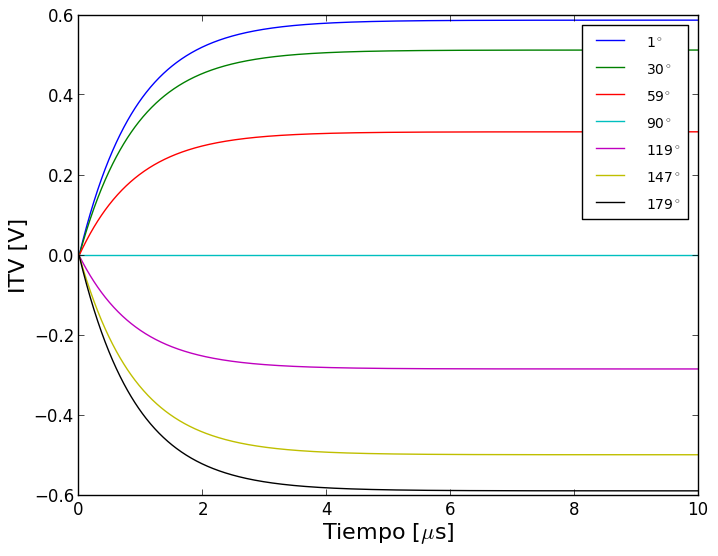
\includegraphics[width=1\textwidth]{itv-time-lin-10-63-40KVm}
%			\caption{63}
%			\label{fig:itv-lin-10-63-40}			
%		\end{minipage}\hfill
%		
%		\begin{minipage}[!h]{.45\paperwidth}
%			\centering
%			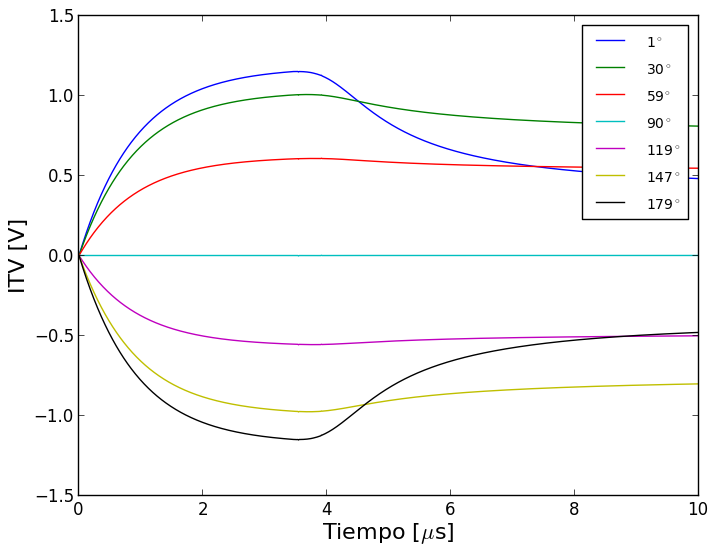
\includegraphics[width=1\textwidth]{itv-time-lin-10-63-80KVm}
%			\caption{63}
%			\label{fig:itv-lin-10-63-80}
%		\end{minipage}\hfill
%	}
%\end{figure}

\newcommand{\itvLinNew}[6]{
\begin{figure}
	\makebox[\textwidth][c] {
		\centering
		\begin{minipage}[!h]{.45\paperwidth}
			\centering
			\includegraphics[width=1\textwidth]{itv-time-lin-#1-#2-#3KVm}
			\caption{ITV al inicio para E=#3KV/m y $\alpha$=#1$\mu$m}
			\label{fig:itv-lin-#1-#2-#3}			
		\end{minipage}\hfill
		
		\begin{minipage}[!h]{.45\paperwidth}
			\centering
			\includegraphics[width=1\textwidth]{itv-time-lin-#4-#5-#6KVm}
			\caption{ITV al inicio para E=#6KV/m y $\alpha$=#4$\mu$m}
			\label{fig:itv-lin-#4-#5-#6}			
		\end{minipage}\hfill
	}
\end{figure}
}

\newcommand{\itvLinNewExtra}[6]{
\begin{figure}
	\makebox[\textwidth][c] {
		\centering
		\begin{minipage}[!h]{.45\paperwidth}
			\centering
			\includegraphics[width=1\textwidth]{itv-time-lin-#1-#2-#3KVm}
			\caption{ITV al inicio para E=#3KV/m y $\alpha$=#1$\mu$m con malla de pocos elementos}
			\label{fig:itv-lin-#1-#2-#3}			
		\end{minipage}\hfill
		
		\begin{minipage}[!h]{.45\paperwidth}
			\centering
			\includegraphics[width=1\textwidth]{itv-time-lin-#4-#5-#6KVm}
			\caption{ITV al inicio para E=#6KV/m y $\alpha$=#4$\mu$m con malla de muchos elementos}
			\label{fig:itv-lin-#4-#5-#6}			
		\end{minipage}\hfill
	}
\end{figure}
}

\itvLinNew{10}{63}{40}{10}{63}{80}
\itvLinNew{10}{63}{120}{10}{63}{160}

%\itvLin{25}{64}{40}
%\itvLin{25}{64}{80}
%\itvLin{25}{64}{160}
%\itvLin{25}{128}{160}

\itvLinNew{25}{64}{40}{25}{64}{80}
\itvLinNewExtra{25}{64}{160}{25}{128}{160}

%\itvLin{50}{64}{40}
%\itvLin{50}{64}{80}
%\itvLin{50}{64}{160}
%\itvLin{50}{64}{200}

\itvLinNew{50}{64}{40}{50}{64}{80}
\itvLinNew{50}{64}{160}{50}{64}{200}

\newpage
\clearpage

%discusión:
%\newpage

\newpage
En las figuras \ref{fig:itv-log-10-63-40} a \ref{fig:itv-log-50-64-200} se graficó lo mismo que en las figuras anteriores, pero sobre todo el pulso de 20 ms y con una escala logarítmica para el tiempo. Se observa que las regiones cercanas al ecuador no dejan de tener un potencial muy cercano a cero durante todo el pulso, mientras que las regiones más alejadas del ecuador terminan alcanzando valores muy similares entre sí: positivos para las regiones del hemisferio hiperpolarizado ($\theta$ menor a 90 grados) y negativos para las regiones del hemisferio depolarizado ($\theta$ mayor a 90 grados).\\

Se observa también en la figura \ref{fig:itv-log-10-63-40} que si el radio de la célula y el campo eléctrico son muy pequeños, el potencial transmembrana no alcanza nunca el valor suficiente como para generar poros y reducir aumentar la conductancia y así el ITV.\\

En las figuras \ref{fig:itv-tita-10-63-40} a \ref{fig:itv-tita-50-64-200} se observa el voltaje transmembrana en función del ángulo $\theta$, en diferentes instantes para diferentes radios y potenciales aplicados. Se observa que la similitud con la fórmula \ref{eq:cos} sólo se observa durante los primeros instantes del pulso, deformándose rápidamente la curva obtenida.

\clearpage

%acá van las imgns itv log

%\newcommand{\itvLog}[3] {
%	\imagen
%		{itv-time-log-#1-#2-#3KVm}
%		{ITV durante el pulso para E = #3KV/m y $\alpha$ = #1um (escala logarítmica)}
%		{itv-lin-#1-#2-#3}
%}

%\newcommand{\itvLogDoble}[6]{
%	\imagenDoble
%		{itv-time-log-#1-#2-#3KVm}{ITV durante el pulso para E=#3KV/m y $\alpha$=#1$\mu$m (escala logarítmica)}{itv-log-#1-#2-#3}
%		{itv-time-log-#4-#5-#6KVm}{ITV durante el pulso para E=#6KV/m y $\alpha$=#4$\mu$m (escala logarítmica)}{itv-log-#4-#5-#6}
%}

\newcommand{\itvLogDoble}[6]{
\begin{figure}
	\makebox[\textwidth][c] {
		\centering
		\begin{minipage}[!h]{.45\paperwidth}
			\centering
			\includegraphics[width=1\textwidth]{itv-time-log-#1-#2-#3KVm}
			\caption{ITV durante el pulso para E=#3KV/m y $\alpha$=#1$\mu$m (escala logarítmica)}
			\label{fig:itv-log-#1-#2-#3}			
		\end{minipage}\hfill
		
		\begin{minipage}[!h]{.45\paperwidth}
			\centering
			\includegraphics[width=1\textwidth]{itv-time-log-#4-#5-#6KVm}
			\caption{ITV durante el pulso para E=#6KV/m y $\alpha$=#4$\mu$m (escala logarítmica)}
			\label{fig:itv-log-#4-#5-#6}			
		\end{minipage}\hfill
	}
\end{figure}
}

%\newpage
%\itvLog{10}{63}{40}
%\itvLog{10}{63}{80}
%\itvLog{10}{63}{120}
%\itvLog{10}{63}{160}
%
%\itvLog{25}{64}{40}
%\itvLog{25}{64}{80}
%\itvLog{25}{64}{160}
%\itvLog{25}{128}{160}
%
%\itvLog{50}{64}{40}
%\itvLog{50}{64}{80}
%\itvLog{50}{64}{160}
%\itvLog{50}{64}{200}

%\clearpage\newpage
\itvLogDoble{10}{63}{40}{10}{63}{80}
\itvLogDoble{10}{63}{120}{10}{63}{160}
\itvLogDoble{25}{64}{40}{25}{64}{80}
\itvLogDoble{25}{64}{160}{25}{128}{160}
\itvLogDoble{50}{64}{40}{50}{64}{80}
\itvLogDoble{50}{64}{160}{50}{64}{200}

%acá van las imgs de itv vs tita

%\newcommand{\itvTita}[3] {
%	\imagen
%		{itv-tita-#1-#2-#3KVm}
%		{ITV según ángulo $\theta$ para E = #3KV/m y $\alpha$ = #1um}
%		{itv-lin-#1-#2-#3}
%}
%\newpage
%\itvTita{10}{63}{40}
%\itvTita{10}{63}{80}
%\itvTita{10}{63}{120}
%\itvTita{10}{63}{120}
%
%\itvTita{25}{64}{40}
%\itvTita{25}{64}{80}
%\itvTita{25}{64}{160}
%\itvTita{25}{128}{160}
%
%\itvTita{50}{64}{40}
%\itvTita{50}{64}{80}
%\itvTita{50}{64}{160}
%\itvTita{50}{64}{200}
%\newpage

%\newcommand{\itvTitaDoble}[6]{
%	\imagenDoble
%		{itv-tita-#1-#2-#3KVm}{ITV según ángulo $\theta$ para E=#3KV/m y $\alpha$=#1$\mu$m}{itv-tita-#1-#2-#3}
%		{itv-tita-#4-#5-#6KVm}{ITV según ángulo $\theta$ para E=#6KV/m y $\alpha$=#4$\mu$m}{itv-tita-#4-#5-#6}
%}

\newcommand{\itvTitaDoble}[6]{
\begin{figure}[!h]
	\makebox[\textwidth][c] {
		\centering
		\begin{minipage}[!h]{.45\paperwidth}
			\centering
			\includegraphics[width=1\textwidth]{itv-tita-#1-#2-#3KVm}
			\caption{ITV según ángulo $\theta$ para E=#3KV/m y $\alpha$=#1$\mu$m}
			\label{fig:itv-tita-#1-#2-#3}			
		\end{minipage}\hfill
		
		\begin{minipage}[!h]{.45\paperwidth}
			\centering
			\includegraphics[width=1\textwidth]{itv-tita-#4-#5-#6KVm}
			\caption{ITV según ángulo $\theta$ para E=#6KV/m y $\alpha$=#4$\mu$m}
			\label{fig:itv-tita-#4-#5-#6}			
		\end{minipage}\hfill
	}
\end{figure}
}

\itvTitaDoble{10}{63}{40}{10}{63}{80}
\itvTitaDoble{10}{63}{120}{10}{63}{160}

\itvTitaDoble{25}{64}{40}{25}{64}{80}
\itvTitaDoble{25}{64}{160}{25}{128}{160}

\itvTitaDoble{50}{64}{40}{50}{64}{80}
\itvTitaDoble{50}{64}{160}{50}{64}{200}

%acá van las imgs de histogramas de poros

\clearpage
\subsection{Poros}

En las figuras 37 a 48 fueron realizados histogramas con la distribución de los radios de los poros grandes generados en distintos instantes y para distintos campos eléctricos aplicados y distintos radios. Sólo fueron graficados los poros grandes (mayores a 1 $\si{\nano\metre}$), que son los de interés. \\

Se observa que si bien se crean muchos poros, éstos se sellan rápidamente con el paso del tiempo: a los 5 ms del pulso en todos los casos la cantidad de poros es mucho menor en instantes anteriores, aunque los pocos poros grandes que siguen existiendo parecen tener mayor radio que la mayoría de los poros en los instantes anteriores. La corta vida de la mayoría de los poros parece deberse a que la alta densidad de los primeros instantes reduce significativamente la conductancia de la membrana, y por lo tanto el ITV necesario para mantener los poros abiertos.

%\newcommand{\histoDoble}[7]{
%	\imagenDoble
%		{hist-radios-#4-#1-#2-#3KVm}{Distribución de radios en los poros grandes para E=#3KV/m y $\alpha$=#1$\mu$m en t=#5}{histo-#1-#2-#3-#4}
%		{hist-radios-#6-#1-#2-#3KVm}{Distribución de radios en los poros grandes para E=#3KV/m y $\alpha$=#1$\mu$m en t=#7}{histo-#1-#2-#3-#6}
%}

\newcommand{\imagenDobleTop}[6]{
\begin{figure}
	\makebox[\textwidth][c] {
		\centering
		\begin{minipage}[t]{.45\paperwidth}
			\centering
			\label{fig:#3}
			\includegraphics[width=1\textwidth]{#1}
			\caption{#2}
		\end{minipage}\hfill
		\begin{minipage}[t]{.45\paperwidth}
			\centering
			\label{fig:#6}
			\includegraphics[width=1\textwidth]{#4}
			\caption{#5}
		\end{minipage}\hfill
	}
\end{figure}
}

\newcommand{\imagenDobleBottom}[6]{
\begin{figure}
	\makebox[\textwidth][c] {
		\centering
		\begin{minipage}[b]{.45\paperwidth}
			\centering
			\label{fig:#3}
			\includegraphics[width=1\textwidth]{#1}
			\caption{#2}
		\end{minipage}\hfill
		\begin{minipage}[b]{.45\paperwidth}
			\centering
			\label{fig:#6}
			\includegraphics[width=1\textwidth]{#4}
			\caption{#5}
		\end{minipage}\hfill
	}
\end{figure}
}

\newcommand{\histoQuad}[3]{
	\newpage
	\imagenDobleTop
		{hist-radios-5e-6-#1-#2-#3KVm}{Distribución de radios en los poros grandes para E=#3KV/m y $\alpha$=#1$\mu$m en t=5\usec}{histo-#1-#2-#3-30e-6}
		{hist-radios-100e-6-#1-#2-#3KVm}{Distribución de radios en los poros grandes para E=#3KV/m y $\alpha$=#1$\mu$m en t=100\usec}{histo-#1-#2-#3-1e-3}
	\imagenDobleBottom
		{hist-radios-1e-3-#1-#2-#3KVm}{Distribución de radios en los poros grandes para E=#3KV/m y $\alpha$=#1$\mu$m en t=1 ms}{histo-#1-#2-#3-8e-3}
		{hist-radios-5e-3-#1-#2-#3KVm}{Distribución de radios en los poros grandes para E=#3KV/m y $\alpha$=#1$\mu$m en t=5 ms}{histo-#1-#2-#3-19e-3}
}

%\histoQuad{10}{63}{40}
%\histoQuad{10}{63}{80}
%\histoQuad{10}{63}{120}
%\histoQuad{10}{63}{160}
%\histoDoble{10}{63}{160}{5e-6}{5$\mu$s}{100e-6}{100$\mu$s}
%\histoQuad{10}{63}{200}
%\histoDoble{10}{63}{200}{5e-6}{5$\mu$s}{100e-6}{100$\mu$s}
%\histoQuad{25}{64}{40}
%\histoQuad{25}{64}{80}
%\histoDoble{25}{64}{80}{5e-6}{5$\mu$s}{100e-6}{100$\mu$s}
%\histoQuad{25}{64}{120}
%\histoQuad{25}{64}{160}
\histoQuad{25}{64}{200}
%\histoQuad{25}{128}{40}
%\histoQuad{25}{128}{80}
%\histoQuad{25}{128}{120}
%\histoQuad{25}{128}{160}
%\histoQuad{25}{128}{200}
%\histoQuad{50}{64}{40}
%\histoQuad{50}{64}{80}
\histoQuad{50}{64}{120}
\histoQuad{50}{64}{160}
%\histoQuad{50}{64}{200}

%\histoDoble{25}{64}{40}{25}{64}{80}
%\histoDoble{25}{64}{120}{25}{64}{160}
%\histoDoble{25}{64}{200}{25}{64}{200}
%\histoDoble{25}{128}{40}{25}{128}{80}
%\histoDoble{25}{128}{120}{25}{128}{160}
%\histoDoble{25}{128}{200}{25}{128}{200}
%\histoDoble{50}{64}{40}{50}{64}{80}
%\histoDoble{50}{64}{120}{50}{64}{160}
%\histoDoble{50}{64}{200}{50}{64}{200}

\clearpage
\subsection{Transporte de especies}
Se graficaron en las figuras 49 a 76 las concentraciones de las especies de interés en escala logarítmica para curvas de nivel r = 0, con los valores iniciales en azul y finales (luego del pulso de 20 ms) en rojo, ambos en escala logarítmica. Los valores de Y centrales corresponden al interior de la célula.

%TODO COMPLETAR NUMEROS AL FINAL!!!!

\begin{itemize}
	\item[\h] 
	Se observa que el ión hidrógeno ingresa muy fácilmente a la célula, obteniendo concentraciones muy altas, con varios órdenes de magnitud mayores a las iniciales. Se observa también que el potencial aplicado incide considerablemente en la densidad de \h en el interior de la célula. 

	\item[\oh]
	Se observa que se logra también el ingreso del grandes cantidades del anión hidróxido a la célula, en particular en las regiones depolarizadas, pero se requiere una campo eléctrico más grande. Por ejemplo, para una célula de 25 $\si{\micro\metre}$ se requieren 120 \kvm para lograr el ingreso en concentraciones significativas.
	
	\item[\na]	
	Se nota que el ingreso del catión sodio a la célula es mucho menor a los anteriores, requiriendo de potenciales mayores, al menos para un solo pulso de 20 ms. Para células de 25 o 50 $\si{\micro\metre}$ de radio se requiere un campo eléctrico de 200 \kvm para lograr un ingreso significativo al interior, obteniendo incluso en ese caso concentraciones menores a las iniciales en las regiones hiperpolarizadas. 
	
	\item[\cl]
	Para células de 25 $\si{\micro\metre}$ o 50 $\si{\micro\metre}$ el anión cloruro ingresa en la célula con campos eléctricos de 160 \kvm  o  200 \kvm, con concentraciones mayores en el segundo caso y concentraciones mayores a las iniciales en toda la célula. Potenciales menores no producen el ingreso en cantidades significativas, e incluso reducen las concentraciones en algunas regiones.
\end{itemize}


% {radio}{malla}{voltaje}
\newcommand{\curvaQuad}[3]{
	\newpage
	\imagenDobleTop
		{curv-H-#1-#2-#3KVm}{Concentraciones de \h en r=0 para E=#3KV/m y $\alpha$=#1$\mu$m}{curva-h-#1-#2-#3}
		{curv-OH-#1-#2-#3KVm}{Concentraciones de \oh en r=0 para E=#3KV/m y $\alpha$=#1$\mu$m}{curva-oh-#1-#2-#3}
	\imagenDobleBottom
		{curv-NA-#1-#2-#3KVm}{Concentraciones de \na en r=0 para E=#3KV/m y $\alpha$=#1$\mu$m}{curva-na-#1-#2-#3}
		{curv-CL-#1-#2-#3KVm}{Concentraciones de \cl en r=0 para E=#3KV/m y $\alpha$=#1$\mu$m}{curva-cl-#1-#2-#3}
}

%\curvaQuad{10}{63}{40}
%\curvaQuad{10}{63}{80}
\curvaQuad{10}{63}{120}
%\curvaQuad{10}{63}{160}
%\curvaQuad{10}{63}{200}
%\curvaQuad{25}{64}{40}
%\curvaQuad{25}{64}{80}
\curvaQuad{25}{64}{120}
\curvaQuad{25}{64}{160}
\curvaQuad{25}{64}{200}
%\curvaQuad{50}{64}{40}
%\curvaQuad{50}{64}{80}
%\curvaQuad{50}{64}{120}
\curvaQuad{50}{64}{160}
\curvaQuad{50}{64}{200}

\newpage\clearpage
\section{Conclusiones y trabajo futuro}

Del trabajo realizado se concluye que es posible ingresar las especies de interés al interior de la célula con la ayuda de un pulso eléctrico para generar poros en la membrana celular e impulsar la migración de las especies. Sin embargo es necesario el uso de campos eléctricos con potencial muy alto para lograr el ingreso del sodio y cloruro a la célula, al menos para un único pulso de 20 ms. \\

Se tiene como primer resultado interesante que una vez alcanzado un potencial aplicado mínimo para generar poros, aplicar potenciales más grandes no aumenta el ITV, sino que sólo reduce el tiempo necesario para que la célula alcance un equilibrio entre el ITV y la densidad y tamaño de poros. Es decir, un mayor voltaje en los electrodos no produce un mayor ITV (una vez alcanzado un valor mínimo).\\

Otro resultado interesante es que la mayoría de los poros grandes creados permanecen abiertos por un tiempo muy pequeño y mucho antes de que las especies estudiadas lleguen a la membrana celular. Esto quiere decir que se produce una permeabilización considerable en la membrana, pero no parece servir al ingreso de especies. Otros tipos de pulsos podrían solucionar este problema, haciendo coincidir la llegada de las especies a la membrana con la creación de los poros.\\

Para el potencial transmembrana al comienzo del pulso se combinan los potenciales obtenidos por la ecuación de potencial eléctrico (\ref{eq:poisson}) con la fórmula \ref{eq:capacit} de carga de un capacitor. Esto significa que los potenciales obtenidos por el método de elementos finitos, usado para el transporte de especies, difieren de los potenciales usados para la creación y crecimiento de poros, usando dos sistemas de ecuaciones dos potenciales diferentes para un mismo instante, pudiendo afectar la precisión de los resultados. Sin embargo el efecto de la capacitancia de la membrana celular solo afecta durante los primeros microsegundos del pulso, como puede observarse en las imágenes de ITV en función del tiempo, en los cuáles el transporte de especies es casi nulo. Dado que la capacitancia de la célula no es muy grande, el valor de $(1 - e^{(-t/\tau)})$ en la fórmula \ref{eq:capacit} se hace rápidamente muy cercano a 1, y el efecto de la capacitancia se vuelve despreciable, eliminándose la discrepancia entre los potenciales usados para resolver la evolución de los poros y el transporte de especies. Sin embrago queda pendiente para el futuro obtener los resultados de potencial en todo el dominio modelando un sistema que tenga en cuenta la capacitancia de la membrana directamente en vez de usar la ecuación \ref{eq:poisson}.\\

También queda pendiente simular distintos tipos de pulsos, en vez de variar sólo su potencial. Es posible que las especies \na y \cl ingresen al interior de la célula en mayores concentraciones o con campos eléctricos menores si se aplican pulsos de mayor duración o si se simulan varios pulsos en vez de uno solo. \\

\begin{thebibliography}{9}

%\bibitem{lamport94}
%  Leslie Lamport,
%  \emph{\LaTeX: a document preparation system}.
%  Addison Wesley, Massachusetts,
%  2nd edition,
%  1994.

\bibitem{puchiar}
	G. Puchiar, T. Kotnik, B. Valič and D. Miklavčič
	\emph{Numerical Determination of Transmembrane Voltage Induced on Irregularly Shaped Cells}
	Annals of Biomedical Engineering
	April 2006, Volume 34, Issue 4, Pages 642-652

\bibitem{fodava}
	Qiong Zheng, Duan Chen and Guo-Wei Wei
	\emph{Second-order Poisson Nernst-Planck solver for ion channel transport}
	Journal of Computational Physics
	Volume 230, Issue 13, 10 June 2011, Pages 5239–5262

\bibitem{krass}
	Wanda Krassowska and Petar D. Filev
	\emph{Modeling Electroporation in a Single Cell}
	Biophysical Journal
	Volume 92, Issue 2, 15 January 2007, Pages 404–417

\bibitem{fem-electro}
	Stanley Humphries, Jr.
	\emph{Finite-element Methods for Electromagnetics}
	2010

\bibitem{fem}
	O.C. Zienkiewicz and R.L. Taylor
	\emph{The Finite Element Method Volume I: The Basis}
	Butterworth-Heinemann,
	5th edition,
	2000

\bibitem{marino}
	Matías Daniel Marino, Dr. Pablo Turjanski, Dr. Nahuel Olaiz
	\emph{Electroporación en el tratamiento de tumores: modelos teóricos y experimentales}
	2013

\end{thebibliography}

\end{document}

%TODO MID indice? otro formato?
%TODO LOW sacar guiones en fin de línea
%TODO LOW ver espacio en pdf
%TODO LOW keywords en español
%TODO LOW latex badbox
